\section{Results}
\label{sec:results}

The results are organised around the lock-in mechanism, not leaderboard
position. They start with accuracy, then follow the answer-, evidence-, and
retrieval-state signals through adaptive retrieval, the strict graph-only
stress test, and the composite audit. Table~\ref{tab:results_snapshot} gives
the running summary; intervals and denominators are kept in the appendix.
The recurring pattern is simple: answer-state metrics rank errors well in
ordinary adaptive runs, but can assign near-zero uncertainty to repeated wrong
answers under lock-in (the failure taxonomy in Table~\ref{tab:failure_taxonomy}). GPS is reported more
cautiously, as a conditional, domain-dependent diagnostic with its usable
denominator shown throughout.

\begin{table*}[t]
\centering
\scriptsize
\caption{%
  Headline accuracy and KG-side diagnostic AUROC.
  Vanilla RAG uses dense retrieval; KG-RAG uses entity-first graph retrieval
  with fallback.
  Accuracy is clean semantic accuracy after provider failures are excluded;
  $n$ counts answered KG rows and $\Delta$ is KG $-$ dense accuracy.
  SRE/SD are answer-state scores, SEU is evidence-state, and GPS is the
  soft-linked, depth-matched graph-support diagnostic, reported in risk
  orientation (lower is stronger support), shown with its
  usable/answered denominator.
  Intervals and denominator details are in
  Appendix~\ref{sec:appendix_reproducibility}.%
}
\label{tab:results_snapshot}
\setlength{\tabcolsep}{3.2pt}
\begin{tabular}{@{}lccccccccp{2.6cm}@{}}
\toprule
Dataset & $n$ & Dense acc. & KG acc. & $\Delta$ & SRE & SD & SEU & GPS (usable) & Main reading \\
\midrule
PubMedQA & 100 & 0.750 & 0.730 & $-0.020$ & 0.64 & 0.70 & 0.59 & -- &
Binary control; GPS abstains (no answer entities). \\
RealMedQA & 223 & 0.950 & 0.946 & $-0.004$ & 0.66 & 0.81 & 0.50 & 0.76 (195/223) &
Clinical parity; GPS calibration domain. \\
HotpotQA & 238 & 0.655 & 0.605 & $-0.050$ & 0.63 & 0.64 & 0.48 & 0.51 (158/238) &
Dense stronger; KG adds anchors and paths. \\
HotpotQA FullWiki & 218 & 0.721 & 0.665 & $-0.056$ & 0.69 & 0.67 & 0.56 & 0.54 (185/218) &
Shared-corpus stress; GPS near chance. \\
2WikiMHQA & 244 & 0.712 & 0.689 & $-0.023$ & 0.65 & 0.69 & 0.64 & 0.38 (182/244) &
Near parity; GPS weak on bridges. \\
MuSiQue & 94 & 0.478 & 0.394 & $-0.084$ & 0.66 & 0.63 & 0.63 & 0.68 (83/94) &
Hard multi-hop; auditable, not competitive. \\
\bottomrule
\end{tabular}
\end{table*}

\begin{figure*}[t]
\centering
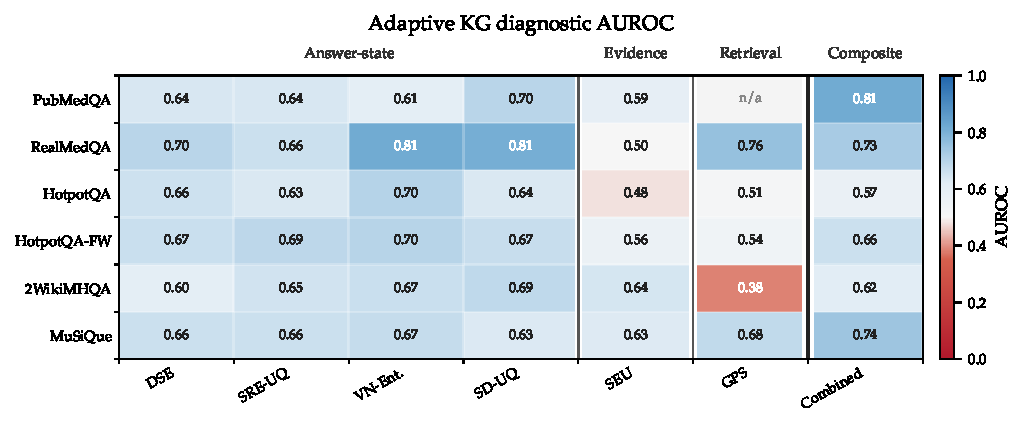
\includegraphics[width=\linewidth]{figures/adaptive_kg_auroc_heatmap}
\caption{%
  \textbf{Adaptive KG-side diagnostic AUROC across the six snapshots,
  grouped by family.}
  Incorrect answers are the positive (risk) class.
  Vertical rules separate the answer-state, evidence-state, and
  retrieval-state families; the derived Combined column is separated because
  it is not a raw metric, but the mean of within-dataset percentile ranks for
  SD-UQ, SEU, and GPS-risk.
  GPS denominators are in Appendix Table~\ref{tab:effective_denominators};
  PubMedQA is undefined because yes/no answers expose no linkable entities.
  The diverging colour scale is neutral at chance ($0.50$), red below, blue
  above.
  Cells are point estimates; bootstrap $95\%$ CIs are in Appendix
  Table~\ref{tab:headline_ci_output}.%
}
\label{fig:adaptive_kg_auroc_heatmap}
\end{figure*}

\subsection{Accuracy: Dense Retrieval Leads; Parity Is the Bar to Clear}
\label{sec:results_accuracy}

Table~\ref{tab:results_snapshot} makes the accuracy picture plain: KG-RAG
trails dense retrieval on five of the six snapshots, with $\Delta$ from
$-0.004$ (RealMedQA, effective parity) to $-0.084$ (MuSiQue), so it neither
beats nor reliably matches dense retrieval on answer quality, and
\system{} is no drop-in accuracy replacement on the harder multi-hop suites.
Where parity holds ($|\Delta| \leq 0.023$ on PubMedQA, RealMedQA, and
2WikiMultiHopQA), the diagnostic question becomes sharp: what does the graph
expose beyond passages?
The adaptive runs test whether KG-RAG preserves accuracy while exposing
anchors, paths, and provenance; the strict graph-only stress test forces
retrieval concentration to probe lock-in.

\begin{table}[t]
\centering
\small
\setlength{\tabcolsep}{6pt}
\renewcommand{\arraystretch}{1.25}
\caption{%
  \textbf{Failure taxonomy for retrieval-augmented generation.}
  Retrieval-state lock-in (top right) is the focal regime: the retrieval state
  is defective while answer-state uncertainty is low.
  Absence lock-in is flagged by retrieval-state abstention; presence lock-in,
  a coherent wrong neighbourhood, remains the hard case.
  At $N{=}5$, $42\%$ of adaptive-KG errors fall in this silent cell
  ($59\%$ dense, $84\%$ strict).%
}
\label{tab:failure_taxonomy}
\begin{tabular}{@{}l >{\raggedright\arraybackslash}p{0.30\linewidth}
                     >{\raggedright\arraybackslash}p{0.30\linewidth}@{}}
\toprule
& \textbf{Retrieval state correct}
& \textbf{Retrieval state wrong / missing} \\
\midrule
\textbf{Low answer-state}  & \cellcolor{goodgreen!15}\textbf{Certified low-risk}
                           & \cellcolor{badred!15}\textbf{Retrieval-state lock-in} \\
\textbf{uncertainty}       & \cellcolor{goodgreen!15}all three families concur
                           & \cellcolor{badred!15}answer-state silent; absence variant flagged by retrieval-state abstention, presence variant open \emph{(this paper)} \\
\addlinespace[0.3em]
\textbf{High answer-state} & \cellcolor{yellow!12}\textbf{Ordinary uncertainty}
                           & \cellcolor{black!6}\textbf{Retrieval failure} \\
\textbf{uncertainty}       & \cellcolor{yellow!12}answer-state flags it
                           & \cellcolor{black!6}answer-state flags it; retrieval-state abstains or shows no support \\
\bottomrule
\end{tabular}
\end{table}


\subsection{Silent Failures Under the Deployable Policies}
\label{sec:results_silent}

Before comparing estimators, the deployable policies already show why
answer-state uncertainty cannot be the whole story.
Table~\ref{tab:silent_failures} reports the \emph{silent-failure rate}: the
fraction of wrong answers whose answer-state uncertainty is exactly zero
(DSE $= 0$ and SD-UQ at its numerical floor), so that no score using only
within-question answer dispersion has a disagreement signal to exploit.
Requiring both conditions is deliberately conservative. DSE $=0$ is the
cluster-count view, where all samples fall in one semantic cluster. The SD-UQ
floor is the embedding-geometry view, where the geometric-mean dispersion
collapses onto the $\varepsilon = 10^{-12}$ stabiliser of
Equation~\eqref{eq:sd_uq}. A row counts as silent only when both views register
no residual variation.
The blind spot belongs to the whole family, not to one estimator: identical
samples contain no disagreement signal for DSE, SD-UQ, VN-Entropy, or any
answer-dispersion variant, though signals outside that family may still help.
Under the deployable policies, $42\%$ of adaptive KG errors and $59\%$ of
dense-retrieval errors are silent, rising to $84\%$ under the strict ablation.
Because the definition requires both semantic unanimity and the SD-UQ numerical
floor at $N=5$, these fractions are conservative symptom counts for this
answer-state family, not exact estimates of every undiagnosable error.

Confidently wrong answers are common in these deployable-policy runs, not only
in the stress regime.
Dense retrieval even produces \emph{more} silent errors than adaptive KG-RAG, so
the phenomenon is not specific to graph retrieval; nor is the dense silence a
low-budget artefact, since on dense 2WikiMultiHopQA the silent rate is still
$68\%$ at $N{=}20$.
The pattern likewise persists under relaxed silent-error floors
(Appendix~\ref{sec:appendix_silent_sensitivity}).

The KG-specific risk is \emph{auditable wrongness}: a silent error can arrive
with matched entities, typed paths, and
provenance anchors, making the system look structurally auditable while it is
wrong. Dense retrieval exposes passages, but not that symbolic trace.
As established in Section~\ref{sec:introduction}, silence is a symptom count;
route logs are needed to diagnose lock-in.

\begin{table}[t]
\centering
\footnotesize
\caption{%
  \textbf{Silent-failure rates with Wilson 95\% intervals.}
  Fraction of wrong answers with zero answer-state uncertainty
  (DSE $=0$ and SD-UQ at its numerical floor), per retrieval policy.
  $n$ is the number of wrong answered rows.%
}
\label{tab:silent_failures}
\setlength{\tabcolsep}{2.5pt}
\begin{tabular}{@{}lccc@{}}
\toprule
Dataset & Dense & Adaptive KG & Strict KG \\
\midrule
PubMedQA    & .84 [.65,.94] (25) & .67 [.48,.81] (27) & --        \\
RealMedQA   & .09 [.02,.38] (11) & .08 [.01,.35] (12) & .73 [.61,.82] (66) \\
HotpotQA    & .59 [.48,.69] (78) & .46 [.36,.56] (94) & --        \\
HotpotQA-FW & .45 [.33,.58] (58) & .18 [.11,.28] (73) & --        \\
2WikiMHQA   & .79 [.67,.87] (61) & .55 [.44,.66] (76) & .90 [.84,.94] (145)\\
MuSiQue     & .51 [.37,.65] (47) & .42 [.30,.55] (57) & --        \\
\midrule
Pooled      & .59 [.53,.65] (280) & .42 [.36,.47] (339) & .84 [.79,.89] (211) \\
\bottomrule
\end{tabular}
\end{table}

In plain terms, an answer-dispersion method cannot recover errors that never
disagree.
At the operational $N{=}5$ budget, a method that only observes sampled-answer
disagreement can recall at most $41\%$ of dense errors, $58\%$ of adaptive
KG errors, and $16\%$ of strict-stress-test errors; the remaining wrong
answers provide no within-question disagreement signal to rank.
That missing observable motivates evidence-state and retrieval-state
diagnostics.

\subsection{Answer-State Metrics Are Strong, but Not Sufficient}
\label{sec:results_output}

Given this blind spot, the next question is how much answer-state estimators
still contribute when retrieval remains adaptive.
In the adaptive runs they remain the strongest default: the AUROC heatmap
(Figure~\ref{fig:adaptive_kg_auroc_heatmap}) shows that answer-side scores have
the clearest overall association with error, especially when retrieval and
decoding still produce meaningful answer variation.
Their limit is equally clear.
When graph routing stabilises the context around a wrong entity or path, answer
disagreement can be low for incorrect answers; the score then measures the
smoothness of the answer surface rather than the reliability of the retrieved
state.
Answer-state uncertainty is therefore a strong default, but not a lock-in
diagnostic.

Within that family, the embedding-geometric scores introduced here are the best
practical answer-side baselines in these low-sample runs.
VN-Entropy and SD-UQ match or beat the imported semantic-entropy and
perturbation baselines on five of the six KG snapshots, with the exception
confined to MuSiQue; the per-dataset AUROCs and intervals are in
Appendix Table~\ref{tab:headline_ci_output}.
The stability split explains why: under high retrieval overlap, DSE falls to
chance while SD-UQ retains signal by removing the question direction before
measuring residual dispersion (Appendix
Table~\ref{tab:within_adaptive_stability}).
SD-UQ is a useful black-box baseline: cheap, embedding-only, and available
without log-probabilities, NLI calls, or model internals.

The verbalised-confidence baseline confirms the boundary rather than removing
it.
Because it asks the model for a probability, it is not blind to silent errors by
construction and recovers part of the clinical silent-error mass.
It still falls to chance on bridge-style lock-in and returns a number without
auditable provenance; the full comparison is in
Appendix~\ref{sec:appendix_verbalized}.

\subsection{The Strict Stress-Test Collapse}
\label{sec:results_collapse}

Answer-state metrics hold up under adaptive retrieval; the question is whether
they survive when retrieval is deliberately concentrated.
The sharpest stress-test signature appears in the strict graph-only regime,
where the retrieved graph state is made more concentrated by disabling dense
fallback, augmentation, reranking, and decomposition, and answer-state
uncertainty becomes a poor guide to correctness.
That answer dispersion falls under forced concentration is expected.
The informative part is what the collapse is made of, which the route
decomposition below recovers.

\begin{figure*}[t]
\centering
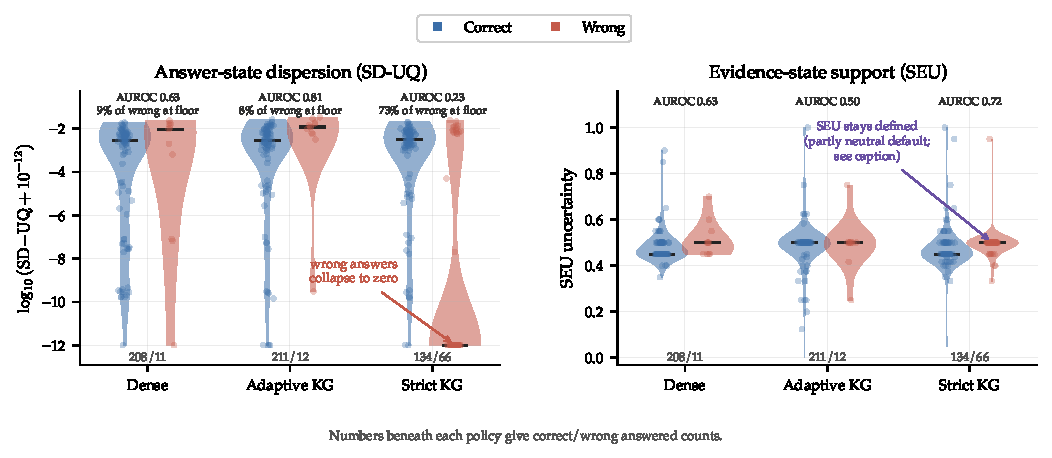
\includegraphics[width=\linewidth]{figures/context_collapse_ablation}
\caption{%
  \textbf{Context collapse in the RealMedQA strict graph-only stress test.}
  Violin/strip distributions are split by correctness, with AUROC printed in
  each panel.
  Under strict retrieval, $73\%$ of wrong answers collapse to the SD-UQ floor
  ($48/66$ vs.\ $1/12$ adaptive; Fisher exact $p = 4\times10^{-5}$).
  SEU remains separated, although Table~\ref{tab:silent_accounting} shows that
  much of the strict signal comes from empty-retrieval defaults.
  The counts beneath each policy are correct/wrong answered rows.
  Strict graph-only retrieval is a mechanism probe.%
}
\label{fig:context_collapse_ablation}
\end{figure*}

\begin{figure*}[t]
\centering
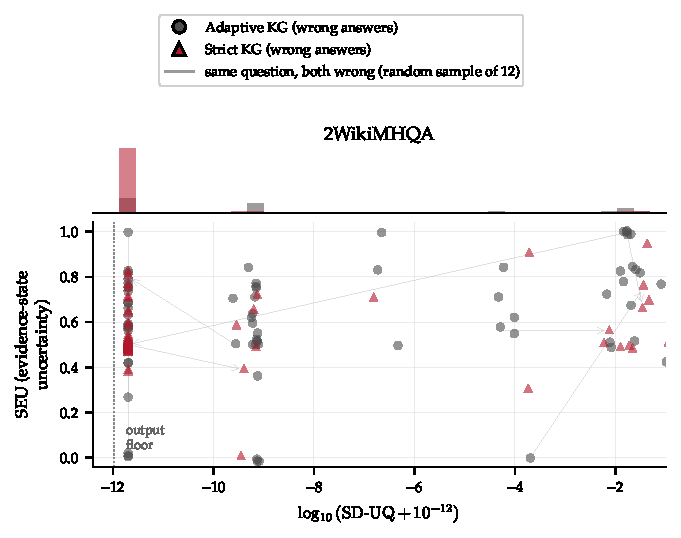
\includegraphics[width=0.92\linewidth]{figures/lockin_migration}
\caption{%
  \textbf{Lock-in as migration into the low-dispersion corner
  (2WikiMultiHopQA).}
  Each point is a \emph{wrong} KG answer, plotted by answer-state dispersion
  (SD-UQ, log scale) and evidence-state uncertainty (SEU), under the
  adaptive policy (grey circles) and the strict graph-only stress test
  (red triangles).
  Grey arrows connect a uniformly random sample of $12$ questions that are
  wrong under \emph{both} policies.
  Under strict retrieval the SD-UQ mass collapses onto the floor while SEU
  remains spread.
  Small vertical jitter is added for legibility.%
}
\label{fig:lockin_migration}
\end{figure*}

Across all paired adaptive--strict questions, $43/196$ RealMedQA questions and
$87/242$ 2WikiMultiHopQA questions move from correct under adaptive KG to
wrong-and-silent under the strict graph-only stress test.
Among questions already wrong but not silent under adaptive KG, another
$2$ RealMedQA and $12$ 2WikiMultiHopQA questions become wrong-and-silent
under strict retrieval; on 2WikiMultiHopQA, $31$ questions remain
wrong-and-silent under both policies.
Thus the stress test does not merely lower accuracy: it moves errors into the
part of the state space where answer-dispersion methods have no disagreement
signal to exploit.

A strict RealMedQA stress test makes the lock-in regime visible directly on the
cleanest parity dataset. As scoped in Section~\ref{sec:introduction}, it is a regime probe:
it shows that lock-in can arise and what the silent signature looks like. The
adaptive rates in Section~\ref{sec:results_silent} measure the deployable-policy
footprint.
It is deliberately harsher: clean KG accuracy falls to $0.670$ on $200$
answered questions, and average within-question chunk overlap rises from
$0.558$ to $0.661$ (Appendix Table~\ref{tab:retrieval_overlap}).
The danger is stability around a wrong symbolic state, not retrieval stability
in itself.
Under that concentrated regime, answer-state ranking largely collapses, as the
strict/adaptive comparison in Figure~\ref{fig:context_collapse_ablation} shows:
DSE AUROC is $0.463$, VN-Entropy AUROC is $0.248$, and SD-UQ AUROC is $0.233$.
On the question subset shared by the two policies, the adaptive-to-strict
SD-UQ gap is $+0.52$ AUROC (paired-bootstrap 95\%~CI $[0.28, 0.73]$,
$n=196$).
The migration plot in Figure~\ref{fig:lockin_migration} shows the mechanism at
question level:
wrong answers migrate from moderate output dispersion under the adaptive
policy into a dense column at the SD-UQ floor under strict retrieval, while
their evidence-support scores remain spread.
That matters because the low-dispersion corner is exactly where answer-state
confidence looks most reassuring and is least informative.
By contrast, SEU reaches $0.721$ AUROC, and GPS reaches $0.746$ on $142/200$
non-abstained rows (Appendix Table~\ref{tab:realmedqa_strict_entity}): the
answer surface goes silent while retrieval-facing scores still rank errors
(GPS here is in its calibration domain).
The contrast holds under an independent Llama-3.3-70B judge ($95.0\%$
agreement, $\kappa = 0.89$): SD-UQ stays collapsed while SEU and GPS still rank
the errors, which same-model self-preference would not explain
(Section~\ref{sec:limitations}).

\paragraph{Route decomposition.}
First, the collapse is not a chunk-level artefact.
An interventional dose-response reduces chunk overlap from $0.67$ to $0.29$,
but leaves SD-UQ AUROC flat ($0.18$) and the silent-error count unchanged
(Appendix~\ref{sec:appendix_doseresponse}).

Second, route logging shows where the silent state lives.
Every silent error in the strict clinical run is an empty-retrieval row
($48/48$ at $n=230$).
Strict anchoring found no usable context, the same empty state recurred across
all five samples, and the generator answered unanimously from parametric
memory.
This points first to removed fallback and vector augmentation as proximate
contributors in this stress run, but the design still changes multiple
components and does not isolate one as the cause.
On the populated-route rows, answer-state ranking is healthy (SD-UQ AUROC
$0.79$).
Much of SEU's apparent survival is mechanical: empty-retrieval wrong rows
receive the all-neutral default $0.5$, which ranks above confidently supported
correct rows; populated-row SEU is only $0.56$.
This is \emph{absence} lock-in, whose simplest reliable flag is the
empty-route/abstention observable, not answer dispersion or evidence
entailment.

Third, the strict 2WikiMultiHopQA run decomposes the same way but leaves a
remainder: $110$ of $130$ silent errors are empty-retrieval, while $20$ ride
populated entity-first routes, wrong-but-coherent neighbourhoods of the
Osireion type (\emph{presence} lock-in), and populated-row SD-UQ stays
degraded there ($0.65$).
Presence lock-in is the harder case: the answer surface and the route
observable are both silent, leaving only evidence-level checks.
It is also a setting where SEU itself proved unreliable (the strict 2-hop
slice), which is why the composite recommendation does not reduce to any single
surviving family.

Under the deployable adaptive policy the silent errors are
mostly presence-like: of the $141$ pooled adaptive silent errors, $99$ carry
recorded route metadata, and among those $89$ ride populated iterative
multi-hop routes with none on the empty-retrieval route, so the
deployable-policy footprint is not an empty-retrieval artefact.
The route claim is limited to the logged subset: the remaining $42$ silent
errors lack route metadata, so their absence/presence mix is not recoverable
from the saved logs.
Decomposing those $141$ adaptive silent errors by which family flags them:
$67$ carry an evidence-state contradiction ($\mathrm{SEU}>0.5$), $127$ carry
weak or absent graph support (GPS $>0.5$ or abstention), and only $7$
($5\%$) remain unflagged by every non-answer family.
A manual audit of these seven (Appendix~\ref{sec:appendix_residue}) finds
mostly benchmark-ambiguous questions, wrong-answer-slot errors, and parametric
conflations rather than confirmable deep presence lock-in whose evidence
\emph{entails} the wrong answer (the Baltic Cup type of
Table~\ref{tab:lockin_gallery}); since retrieved chunk texts are not archived,
that deceptive type cannot be confirmed from logs.

Flagging the cases where all three families fail, with SEU and GPS both near
zero on a wrong answer, would need exactly what the logs lack here: archived
chunk text for cross-passage contradiction mining, and relation-level path
faithfulness to check that the connecting path uses the relation the question
asked for rather than a locally coherent but wrong one.
Both are concrete, retrieval-replay-only extensions, not new theory.
Table~\ref{tab:silent_accounting} makes the accounting explicit.

\begin{table*}[t]
\centering
\scriptsize
\caption{%
  \textbf{Silent-error accounting from saved logs.}
  Buckets are mutually exclusive and apply only to wrong answered rows.
  ``Max answer recall'' is the structural upper bound for any
  answer-dispersion-only detector at the $N{=}5$ budget: silent wrong answers
  contain no sampled-answer disagreement signal.
  Empty denotes absence lock-in; Pop.+SEU and Pop.+GPS are populated-route
  silent errors flagged by evidence or graph-support signals.
  Unflagged is the residue with no non-answer-family flag.%
}
\label{tab:silent_accounting}
\setlength{\tabcolsep}{3pt}
\begin{tabular}{@{}lrrrrrrrr@{}}
\toprule
Run & Wrong & Silent & Max answer recall & Empty & Pop.+SEU & Pop.+GPS & Route-unk.+flag & Unflagged \\
\midrule
Adaptive KG pooled & 339 & 141 & .58 & 0 & 40 & 44 & 50 & 7 \\
Strict KG pooled   & 211 & 178 & .16 & 158 & 13 & 6 & 0 & 1 \\
RealMedQA strict   & 66  & 48  & .27 & 48  & 0  & 0 & 0 & 0 \\
2WikiMHQA strict   & 145 & 130 & .10 & 110 & 13 & 6 & 0 & 1 \\
\bottomrule
\end{tabular}
\end{table*}
Under this deterministic graph-only regime, answer-surface uncertainty can
cease to track correctness.
Which signal survives depends on the variant: route or abstention observables
for absence, and evidence-level checks, imperfectly, for presence.

The same pattern appears on the newer 2WikiMultiHopQA $n=250$ run when the
three retrieval policies are compared on the identical question subset; the
full hop-stratified breakdown is in Appendix
Table~\ref{tab:twowiki_hopwise_diagnostics}.
The adaptive KG policy is the appropriate deployment comparison: it remains
close to dense retrieval overall (clean accuracy $0.689$ versus $0.712$) and
matches dense retrieval on the 4-hop slice.
On the 4-hop slice, strict graph-only KG has zero clean accuracy while
SD-UQ and VN-Entropy both collapse essentially to zero: the answer surface is
stable precisely when the retrieved graph state has become wrong enough to
make every answer fail.
Low answer-state uncertainty is not intrinsically bad. In the dense 4-hop row,
SD-UQ is also near zero, but VN-Entropy remains non-zero and clean accuracy
stays high, so the collapse signature is the joint collapse of SD-UQ and
VN-Entropy together with failed answers, not low SD-UQ alone.
For KG-RAG, answer agreement must therefore be read alongside evidence- and
retrieval-state diagnostics when the symbolic state has concentrated around a
wrong neighbourhood.
Per-question support comes from a dedicated graph-state diversity run on
HotpotQA-FullWiki that logged per-sample overlap for the seed entities, paths,
subgraph, and chunks ($n=221$ answered, $74$ wrong; Table~\ref{tab:diversity_run}).
Across the $N=5$ samples the retrieval state is highly stable
(seed-entity Jaccard $0.99$; path, subgraph, and chunk $0.58$--$0.65$), so
repeated samples really do condition on nearly the same state; and among
\emph{wrong} answers more overlap predicts lower dispersion
(path/subgraph/chunk Spearman $\rho = -0.30$/$-0.23$/$-0.24$, all $p<0.05$,
$n=74$; the seed-entity coupling is null only because seed overlap saturates
near $1.0$, leaving no variance to correlate against).
The archived traces show the same sign, carried by the bridge-style
2WikiMultiHopQA trace ($\rho = -0.32$, $p = 0.01$, $n = 60$; pooled
$\rho = -0.27$), with no comparable pattern on the dense side.
These analyses support the mechanism without identifying it causally
(Appendix~\ref{sec:appendix_diversity}, \ref{sec:appendix_concentration};
the per-dataset concentration facets are in Figure~\ref{fig:concentration_facets}).

\begin{table}[t]
\centering
\scriptsize
\caption{%
  \textbf{Per-sample graph-state diversity on the dedicated HotpotQA-FullWiki
  run} ($n=221$ answered, $74$ wrong).
  \emph{Stability} is the mean (median) pairwise Jaccard overlap across the
  $N=5$ samples per question, by retrieval-state family.
  \emph{Coupling} is the correlation between that per-question overlap
  and answer-state dispersion (SD-UQ) among wrong answers ($n=74$), reported as
  Spearman's $\rho$ with its two-sided $p$-value; a negative
  value means more overlap goes with less dispersion, the lock-in prediction.%
}
\label{tab:diversity_run}
\begin{tabular}{@{}lcccc@{}}
\toprule
 & \multicolumn{2}{c}{Stability (Jaccard)} & \multicolumn{2}{c}{Coupling vs SD-UQ} \\
\cmidrule(lr){2-3}\cmidrule(lr){4-5}
Family & Mean & Median & $\rho$ & $p$ \\
\midrule
Seed entity & $0.99$ & $1.00$ & $+0.09$ & $0.47$ \\
Path        & $0.58$ & $0.58$ & $-0.30$ & $0.009$ \\
Subgraph    & $0.64$ & $0.63$ & $-0.23$ & $0.048$ \\
Chunk       & $0.65$ & $0.65$ & $-0.24$ & $0.037$ \\
\bottomrule
\end{tabular}
\end{table}

HotpotQA supplies a useful counterweight.
Dense retrieval leads on accuracy ($0.655$ vs.\ $0.605$; FullWiki $0.721$ vs.\
$0.665$) while answer-state AUROCs stay healthy on both systems and GPS is only
weakly discriminative ($0.51$ and $0.54$ usable-row AUROC; Appendix
Table~\ref{tab:hotpot_fullwiki_stress}).
These runs mark the thesis boundary rather than contradicting it: when dense
retrieval already has a compact, well-indexed candidate set, graph
organisation adds provenance and traceability but the current policy does not
improve answer quality or retrieval-state ranking.

Figure~\ref{fig:selective_prediction} reframes the same results as a
selective-prediction problem, the clinical form of the uncertainty question:
if a diagnostic score is high, should the system answer, broaden retrieval,
or send the case to review?
In ordinary adaptive runs, answer-side scores often give the cleanest
rejection signal.
In lock-in regimes, SEU and GPS have to be read as provenance checks rather
than weaker versions of answer-state entropy.

The key appendix row is the strict graph-only 4-hop slice
($n=58$, clean accuracy $0.000$, SD-UQ mean $0.000$, VN-Entropy mean $0.000$).
AUROC is intentionally left undefined because all 58 clean answers are
incorrect, so the evidence is the conjunction of zero accuracy and collapsed
output scores, not a forced ROC statistic: a mechanism demonstration, not a
deployment result.

\subsection{Evidence-State Metrics Add Support-Level Signal}
\label{sec:results_grounding}

If the answer surface goes silent under concentration, the next
question is whether the retrieved evidence itself betrays the error.
Evidence-state measures ask whether the retrieved passages support the answer
that was produced, not whether sampled answers agree; this matters especially
in high-accuracy or near-parity settings where the deployment question is
whether the answer can be justified by retrieved evidence.

The aggregate evidence-state signal is weaker than the answer-state family as
a global ranker, but complementary rather than redundant.
SEU's survival under lock-in is dataset-dependent. It reaches $0.721$
AUROC on the strict RealMedQA ablation, although the route decomposition in
Section~\ref{sec:results_collapse} shows that much of this signal comes from
the all-neutral default over empty-retrieval rows, not from genuine entailment.
On the strict 2WikiMultiHopQA 2-hop slice, it falls below chance
(Appendix Table~\ref{tab:twowiki_hopwise_diagnostics}). Evidence support is
therefore useful, but not uniformly robust to retrieval concentration.
The 2-hop failure has a concrete mechanism: on bridge questions the strict
policy retrieves passages about the wrong-but-coherent anchor, and those
passages weakly \emph{entail} the wrong answer drawn from that neighbourhood
rather than contradicting it, so low SEU and incorrectness coincide.
On the clinical corpus, the contradiction is visible in the retrieved text
itself; SEU survives there for this reason.
SEU is also low-resolution where retrieval returns long, loosely-relevant
chunks: on the adaptive RealMedQA run, $74\%$ of answered rows receive the
all-neutral value $0.5$ because no retrieved chunk is judged to entail or
contradict the answer, which explains the chance-level adaptive AUROC there.
In that regime the score is silent rather than wrong; sentence-level
entailment scoring is the plausible refinement, but it requires re-running
retrieval rather than replaying logs.
The selective-prediction curves in Figure~\ref{fig:selective_prediction}
and the fixed-coverage operating points in Appendix
Table~\ref{tab:operating_points} give the same lesson in decision form.

\begin{figure*}[t]
\centering
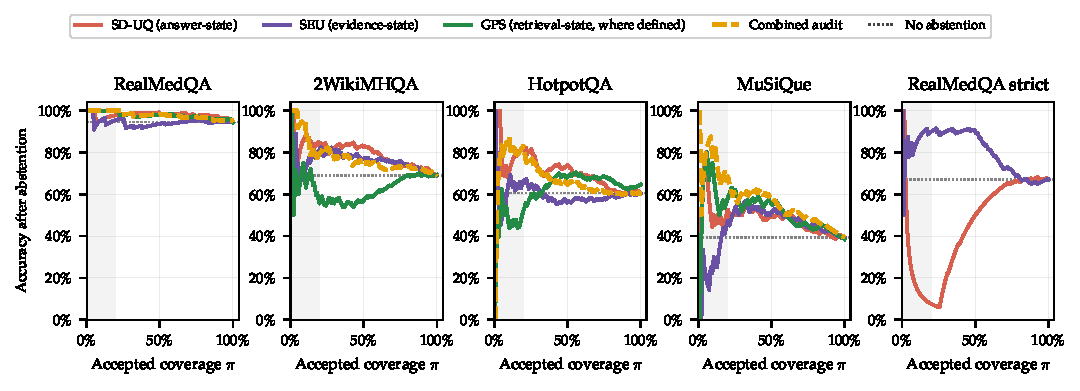
\includegraphics[width=\linewidth]{figures/coverage_accuracy}
\caption{%
  \textbf{Selective prediction with different KG-side diagnostic families},
  including the RealMedQA strict ablation (rightmost panel).
  Curves sort answered KG-RAG queries by increasing uncertainty and then
  report the accuracy retained at each accepted coverage level; the dotted
  line is the no-abstention accuracy and the shaded band marks the noisy
  $<20\%$-coverage region.
  The strict panel carries the decision-form headline: SD-UQ gating
  \emph{inverts}: accepting the lowest-dispersion answers first means
  accepting the silent wrong mass, while SEU gating climbs toward $90\%$.
  GPS and the combined audit are omitted from the strict panel because GPS
  comes from post-hoc replay rather than row-level logs.%
}
\label{fig:selective_prediction}
\end{figure*}
Under the adaptive policy, gating on SD-UQ alone is the strongest simple
abstention rule; under the strict clinical ablation that rule becomes
uninformative ($0.338$ error at $80\%$ coverage against a $0.330$
no-abstention base) while SEU gating cuts the residual error to $0.269$, an
$18\%$ relative reduction in the regime where the answer surface is silent.
The useful diagnostic changes with the retrieval regime; a single global
ranking hides that switch.

\subsection{Where Retrieval-State Diagnostics Work and Where They Do Not}
\label{sec:results_structural}

Retrieval-state diagnostics ask the complementary question: when does the graph
state itself reveal weak support?
GPS behaviour is domain-dependent.
On the clinical shared-corpus setting where its two hyperparameters were
calibrated, it is a useful error ranker ($0.76$ adaptive, $0.75$
strict); on the held-out open-domain suites transfer is uneven (MuSiQue $0.68$
with per-question depth, but HotpotQA $0.51$, FullWiki $0.54$, and
2WikiMultiHopQA $0.38$ near or below chance).
A sensitivity replay over $\tau\in\{0.50,\ldots,0.70\}$ and
$\gamma\in\{0.2,\ldots,1.0\}$ leaves the held-out open-domain GPS AUROCs
essentially unchanged (SD $\leq 0.018$ for HotpotQA, FullWiki,
2WikiMultiHopQA, and MuSiQue; Appendix Table~\ref{tab:gps_sensitivity}), so
the weak 2WikiMultiHopQA ranking is not a threshold/decay artefact.
GPS scores graph support for the generated answer, not correctness.
It can therefore rate a wrong-but-coherent neighbourhood as low risk: in the
Baltic Cup case of Table~\ref{tab:lockin_gallery}, the wrong entity is reachable,
GPS is $0.00$, SEU is $0.00$, and the answer surface has near-zero dispersion.
The decomposition makes that failure visible but does not solve it.
Retrieval-state AUROC is therefore computed only on rows with linkable answer
entities, with linking failures reported as abstentions
(Table~\ref{tab:results_snapshot}). GPS contributes most reliably as an
abstention record, usable denominator, and trace-level support check; its scalar
ranking is useful only in validated domains.
A fixed-bin reliability check makes the same point without AUROC:
RealMedQA error rates rise from $0/39$ in the lowest GPS-risk bin to $6/42$
in the highest, but the open-domain bins are not monotone, especially on
2WikiMultiHopQA (Appendix Table~\ref{tab:gps_reliability_bins}).

Soft answer-entity linking substantially reduces the abstention cost: usable
denominators now cover most answered rows (e.g.\ $185/218$ on HotpotQA
FullWiki, up from $69$ under pure surface matching), with the per-dataset
values in Table~\ref{tab:results_snapshot} and Appendix
Table~\ref{tab:effective_denominators}.
PubMedQA still abstains completely because binary answers expose no answer
entities, a structural boundary rather than a linking failure.
Coverage repair is not ranking repair: the held-out AUROCs above
show that making more rows scoreable does not by itself make the score a
better error ranker.
Closing the open-domain ranking gap most plausibly requires relation-level
path faithfulness, checking that the connecting path uses the relation the
question asked for, rather than further entity-linking improvements.
The 2WikiMultiHopQA replay shows the problem directly.
The adaptive $n=250$ run gives GPS AUROC $0.38$ on $182/244$ usable rows because
$71\%$ of correct adaptive answers have their gold entity unreachable in the
retrieved subgraph, against $45\%$ of wrong ones.
Here GPS is not miscalibrated; it is exposing a retrieval policy that can make
the wrong answer reachable while leaving the gold answer outside the graph state.

The post-hoc replay on the full $n=230$ answer log, recomputing only
GPS, without rerunning generation or
retrieval, raises KG-side coverage from $97/223$ to $195/223$ and AUROC from
$0.47$ to $0.76$ (Appendix Table~\ref{tab:realmedqa_replay}); the same replay
reaches $0.89$ on the dense side.
RealMedQA is the calibrated case: it shows what retrieval-state scoring can
deliver on a clinical shared corpus, while the held-out rows above show the
generalisation limit.

\subsection{Concrete Cases}
\label{sec:results_cases}

The aggregate AUROCs and route statistics summarise behaviour across
questions; the Osireion trace in Figure~\ref{fig:lockin_trace} shows
how the three families interact on a single answer, and is deliberately not a
case where every diagnostic succeeds.
Answer-state uncertainty is at its floor ($\mathrm{DSE}=0$,
$\mathrm{SD\text{-}UQ}\approx 0$) because all samples repeat the wrong entity;
GPS is low ($0.44$), so it does not flag the case: the wrong entity is
reachable in the retrieved graph. This is correct behaviour for a
risk-oriented support diagnostic, but not a truth guarantee. SEU alone raises
risk ($1.0$), because every retrieved chunk
contradicts the confident, graph-coherent answer.
The practical meaning of path faithfulness is therefore that the graph can make
a wrong reasoning chain visible even when the scalar retrieval-state score
reports low risk, provided the evidence-support head is read with it; the full
per-case audit readout is in Appendix Table~\ref{tab:path_faithfulness_case}.
A consolidated case gallery, with seven verified lock-in failures, four KG
successes, and per-case diagnostic readouts, is in
Appendix~\ref{sec:appendix_cases} (Table~\ref{tab:lockin_gallery}).

\subsection{The Composite-Suite Thesis}
\label{sec:results_composite}

Finally, if the three families answer different diagnostic questions, the
decision layer should not collapse them too early.
They also barely move together, which is the quantitative case
for keeping them apart; Appendix Figure~\ref{fig:family_disagreement} shows this
for the adaptive KG setting.
Across the six-snapshot heatmap suite ($n=803$ pooled non-abstained KG rows),
the pooled KG-side Spearman correlations are small to modest:
$\rho=0.03$ for SD-UQ versus SEU, $\rho=-0.27$ for SD-UQ versus GPS, and
$\rho=-0.10$ for SEU versus GPS; the pooled family-disagreement scatter is in
Appendix Figure~\ref{fig:family_disagreement}.
The three scores therefore carry partly separate diagnostic signal, even if low
correlation alone cannot identify distinct latent causes.
Because GPS is a graph-support diagnostic reported in risk orientation rather
than an information-theoretic uncertainty score, lower GPS means stronger local
graph support for the generated answer, so the negative SD-UQ--GPS sign should
not be read as a universal risk law.

If all three families tracked the same object, a single scalar confidence
score would suffice; they do not, and expose different failure modes.
The recommendation is a composite diagnostic suite, not a single-metric
leaderboard. In practice, a low answer-state score should not override a
retrieval-state abstention, a fragile graph path, or high evidence
contradiction; such discordant profiles are good candidates for abstention,
broader retrieval, or human review.
A deliberately simple percentile-rank audit score, averaging SD-UQ, SEU, and
GPS-risk within each dataset, shows how the three families can feed a decision
layer. It is uneven, but useful where answer dispersion is coarse
(e.g.\ PubMedQA Combined $0.813$ vs.\ SD-UQ $0.699$;
Appendix~\ref{sec:appendix_composite},
Table~\ref{tab:composite_audit_score}).

\paragraph{A conjunctive low-risk audit rule.}
The conservative rule is narrow by design: it selects $7.7\%$ of answers at
$91.9\%$ accuracy ($86$ of $1{,}117$ questions), against a $69.7\%$ base rate.
It treats a response as low-risk only when all three families concur: low
answer-state uncertainty (SD-UQ in the lower half of its dataset
distribution), non-contradictory evidence support ($\mathrm{SEU} \leq 0.5$),
and defined, present retrieval-state support ($\mathrm{GPS} \leq 0.5$).
The cutoffs are label-free: SEU and GPS use their fixed neutral point ($0.5$),
and SD-UQ uses the dataset median. A deployment would choose its own coverage
point on held-out calibration data.
On the clinical target domain it selects $22\%$ of answers at $100\%$ precision
under the automated judge ($48/48$ correct), a figure that would need
human-expert confirmation before any clinical use (Section~\ref{sec:ethics}).
The same fixed policy is applied unchanged to every dataset. Table~\ref{tab:certificate_perds}
therefore acts as the cross-dataset generalisation view: it reports
per-dataset coverage, precision with Wilson intervals, and recall. Recall is
included because a high-precision selection rule is trivial without it.
Coverage is structurally limited: the rule cannot select answers
with no linkable answer entity (binary, numeric, or label-space answers, where
GPS abstains by construction), so on those formats it defers rather than
selects, and a deployment would need a separate fallback.
The conjunction beats matched-coverage scalar gates: SD-UQ alone gives
$81.4\%$ precision at the same coverage, and the percentile-rank combined score
gives $88.4\%$. A dataset-stratified Mantel--Haenszel check gives the same
direction (odds ratio $3.39$, bootstrap 95\% CI $[1.64, 10.99]$;
Appendix~\ref{sec:appendix_reproducibility}).
The rule is exploratory and domain-conditional. It is strongest on the clinical
target domain, thin-coverage on the harder multi-hop sets, and undefined for
label-space answers. Its purpose is to show what the three-family decomposition
makes possible as an audit policy.

\begin{table}[t]
\centering
\scriptsize
\caption{%
  Per-dataset conjunctive audit-rule behaviour on the adaptive KG runs.
  Recall is the fraction of all \emph{correct} answers selected by the rule;
  it is high-precision and low-recall by design,
  Wilson intervals expose the small denominators,
  and its utility presumes that unselected answers are routed to ordinary
  confidence handling or review rather than discarded.%
}
\label{tab:certificate_perds}
\setlength{\tabcolsep}{2.5pt}
\begin{tabular}{@{}lrrcr@{}}
\toprule
Dataset & Selected & Prec. & 95\% CI & Recall \\
\midrule
PubMedQA & 0/100 (0\%) & -- & -- & 0.00 \\
RealMedQA & 48/223 (22\%) & 1.000 & [0.926, 1.000] & 0.23 \\
HotpotQA & 6/238 (3\%) & 0.833 & [0.436, 0.970] & 0.04 \\
HotpotQA-FW & 26/218 (12\%) & 0.808 & [0.621, 0.915] & 0.14 \\
2WikiMHQA & 4/244 (2\%) & 1.000 & [0.510, 1.000] & 0.02 \\
MuSiQue & 2/94 (2\%) & 0.500 & [0.095, 0.905] & 0.03 \\
\midrule
Pooled & 86/1117 (7.7\%) & 0.919 & [0.841, 0.960] & 0.10 \\
\bottomrule
\end{tabular}
\end{table}
The only data-dependent threshold (the per-dataset SD-UQ median)
survives held-out evaluation: computing it on a random half of each dataset
and applying the rule to the other half gives $91.8\%$ mean precision
(5th--95th percentile $86.7$--$97.4\%$ over $200$ splits) at unchanged
coverage, so the in-sample number is not threshold overfitting.
Per-dataset behaviour exposes both cautionary cases: 2WikiMultiHopQA
selects only four answers ($2\%$ coverage) despite weak GPS ranking, while
MuSiQue selects two answers at only $50\%$ precision.
Per-domain validation is mandatory.
Coverage is bounded mainly by GPS definability and SEU neutrality, so
the refinements above (soft linking already; sentence-level entailment next)
are the most direct route to higher audit-rule coverage.
A simple learned alternative does not transfer better in this fixed-subset test:
leave-one-dataset-out logistic gating selects $7.5\%$ of answers at $85.7\%$
precision. With three scalar features and substantial cross-dataset shift,
conjunctive gating remains the more auditable policy.
